\documentclass[11pt]{report}
\usepackage[dutch]{babel}
\usepackage{a4}
\usepackage{latexsym}
\usepackage[
        colorlinks=true,
	linkcolor=zwart,
        pdftitle={Electronic Scout},
        pdfsubject={Tekst Beeld en Representatie},
        pdfauthor={Thomas Veerman, Martijn Vermaat, Bram Voortman}
]{hyperref}
\usepackage{graphicx}
\usepackage{color}
\definecolor{zwart}{rgb}{0,0,0}

\title{Electronic Scout}
\author{
	Thomas Veerman \\ tveerman@cs.vu.nl
	\and
	Martijn Vermaat \\ mvermaat@cs.vu.nl
        \and
        Bram Voortman \\ jvoortm@cs.vu.nl
}
\date{Amsterdam, Vrije Universiteit, 22 april 2003}

\begin{document}

\maketitle

\thispagestyle{empty}
\thanks{
	Wij bedanken de RAI Amsterdam, AHOY Rotterdam en het VU Academisch Ziekenhuis Amsterdam voor de verleende toegang en toestemming voor het vastleggen van bewegwijzering op foto's.
	\\
	\\
	\\
	\\
	\\
	Van dit document is een versie in PDF formaat te vinden op:\\
	\verb|http://www.cs.vu.nl/~mvermaat/things/vu/tbr2003.xhtml|
}

\begin{abstract}
In dit document presenteren wij ons onderzoek naar de bestaande bewegwijzering binnen de RAI Amsterdam en het ontwerpen van een alternatief systeem.

In het eerste hoofdstuk definieren we ons onderzoeksgebied en het doel van het onderzoek. We beschrijven in het tweede hoofdstuk alle stakeholders. Om een beeld te krijgen van bestaande systemen bekeken en evalueerden we de bewegwijzering in de RAI Amsterdam, AHOY Rotterdam en het VU Academisch Ziekenhuis Amsterdam in de hoofdstukken 3 en 4.

Op basis van de opgedane kennis presenteren we in hoofdstuk 5 een voorstel voor een nieuwe bewegwijzering binnen de RAI Amsterdam. Tenslotte evalueren we dit voorstel het laatste hoofdstuk.
\end{abstract}

\tableofcontents

\listoffigures

\chapter{Domein van onderzoek}

Ons onderzoek zal zich richten op de RAI, het grote beurscomplex in Amsterdam Oud-Zuid. We onderzoeken hier de bewegwijzering binnen en rond de verschillende hallen die als doel heeft de weg te kunnen vinden binnen het complex.

We laten de bewegwijzering die als doel heeft de weg te kunnen vinden in het stadsdeel of zelfs binnen heel Amsterdam buiten beschouwing. Dit zijn bijvoorbeeld bordjes binnen de hallen die het station of de tramhalte wijzen, of bordjes in het station die de richting aangeven van de beursgebouwen.


\section{Situaties en activiteiten}

Het complex wordt van dag tot dag voor verschillende doeleinden gebruikt. Zo zijn er regelmatig grote evenementen in de hallen, met als bekendste voorbeelden de \emph{AutoRAI}, de \emph{FietsRAI} en de \emph{Hiswa}. Andere wisselende activiteiten zijn symposia en congressen.

Daarnaast is er nog een veelheid aan permanente activiteiten te vinden in het complex, zoals restaurants, toiletten en parkeerplaatsen.

Bij iedere activiteit hoort een scala van \emph{meta-activiteiten}, zoals kaartverkoop, schoonmaken, opbouwen en afbreken van stands en informatieverstrekking. Dit alles wordt in veel gevallen ondersteund door de aan- en afvoer van goederen.


\section{De rol van representaties}

De bewegwijzering in de RAI is op de eerste plaats van groot belang bij grote evenementen en andere wisselende activiteiten. Een aanzienlijk deel van deze bewegwijzering zal per activiteit van inhoud verschillen. Er is op bijvoorbeeld een computerbeurs bewegwijzering nodig om de verschillende stands te kunnen vinden. Op het moment dat er in deze hal(len) een nieuw evenement gehouden wordt is deze bewegwijzering niet nuttig meer.
Maar er is ook een deel dat permanent aanwezig moet zijn in het complex. Denk hierbij vooraal aan bewegwijzering naar de verschillende hallen, in- en uitgangen en andere delen van de RAI.

Voor de permanente activiteiten in de RAI is ook bewegwijzering nodig. Iedereen moet de restaurants, toiletten en parkeerplaatsen kunnen vinden en het liefst ook vanaf iedere locatie binnen de RAI. Hierbij moeten we bedenken dat ieder restaurant en iedere parkeerplaats altijd gevonden moet kunnen worden, maar dat in het algemeen bewegwijzering naar een toiletruimte (de dichtstbijzijnde) voldoende zal zijn.

Ook voor de meta-activiteiten is bewegwijzering nodig. Mensen moeten weten waar de kaartjes gekocht dienen te worden, schoonmakers moeten de weg kunnen vinden, aan- en afvoerders van goederen moeten weten waar ze moeten zijn, etc.


\section{Doel van onderzoek}

Het doel van ons onderzoek is het ontwerpen van een nieuwe representatie voor bewegwijzering binnen multifunctionele gebouwen. Door te kijken naar bestaande representaties stellen we verbeteringen voor. De door ons ontworpen representatie staat voor een electronische systeem.


\chapter{Stakeholders}


\section{Bezoekers van evenementen} \label{sectie:stkh_bzkr}

Zonder bezoekers geen evenement. Bezoekers hebben niet tot ieder deel van de RAI toegang, maar zijn wel de belangrijkste stakeholders. Wanneer ze de weg niet goed kunnen vinden zal dat de beleving negatief be\"\i nvloeden en komen ze volgend jaar niet terug.

De bezoekers van evenementen zoeken meer dan alleen stands en symposia. Ze willen tussendoor ook het toilet en het restaurant kunnen vinden.

We moeten goed bedenken dat deze stakeholder niet iedere dag de RAI bezoekt en dus de bewegwijzering snel moet begrijpen.

\subsection*{Taken}

\begin{itemize}
\item Faciliteiten zoals WC, garderobe en restauratie vinden.
\item Evenementen en onderdelen daarvan zoals stands vinden.
\item Te weten komen waar hij/zij zich bevindt.
\item Uitgangen vinden.
\end{itemize}


\section{Werknemers van de RAI}

De bewegwijzering voor deze stakeholder moet overal in het complex aanwezig zijn. Het is een minder belangrijke stakeholder dan de bezoeker van evenementen, in die zin dat de RAI werknemer betaald wordt voor zijn werk en de bewegwijzering minder hard zal afstraffen op gebreken.

Een RAI werknemer komt in tegenstelling tot de bezoeker van een evenement  vaker op het complex en zal er daarom bekender mee zijn. Bewegwijzering is dus in veel gevallen minder belangrijk voor deze stakeholder. Maar, er zijn natuurlijk altijd nieuwe werknemers, of werknemers die een deel van het complex bezoeken waar ze gewoonlijk niet werken.

\subsection*{Taken}

\begin{itemize}
\item Kamers van andere werknemers vinden.
\item Faciliteiten zoals WC, garderobe en restauratie vinden.
\end{itemize}


\section{Klanten van de RAI}

Met de klanten van de RAI bedoelen we de organisatoren van evenementen en de eventuele werknemers hiervan. Deze moeten weten wat de indeling is van het complex, zodat ze hun evenement kunnen indelen.

\subsection*{Taken}

\begin{itemize}
\item Verschillende hallen en zalen vinden.
\item Kamers van andere werknemers vinden.
\item Faciliteiten zoals WC, garderobe en restauratie vinden.
\end{itemize}


\section{Leveranciers van goederen}

Met leveranciers van goederen bedoelen we mensen die bijvoorbeeld de post komen brengen, het complex van eten en drinken voorziet, etc. Voor hen is het belangrijk dat ze weten waar bijvoorbeeld hun aanleverpunt is.

\subsection*{Taken}

\begin{itemize}
\item Verschillende hallen en zalen vinden.
\item Locatie voor afgifte van goederen en magazijn vinden.
\end{itemize}


\section{Beheerders van de bewegwijzering}

Er zijn uiteraard ook een of meerdere personen (werkend voor de RAI) die de bewegwijzering moeten beheren. Eigenlijk valt hier ook het opzetten van het systeem onder, de eerste keer. Maar misschien is het onderhouden ervan nog belangrijker. In hoeverre de bewegwijzering binnen de beursgebouwen aangepast moet worden bij verschillende activiteiten moet onderzocht worden, net zoals welke rol de organisatie van deze activiteiten daar in spelen.

\subsection*{Taken}

\begin{itemize}
\item Installeren van het bewegwijzering systeem.
\item Aanpassen van bewegwijzering systeem.
\end{itemize}


\chapter{Overzicht bestaande representaties}

Om te kijken wat er in de praktijk gebruikt wordt op het gebied van bewegwijzering in multifunctionele gebouwen zijn we gaan kijken in de RAI Amsterdam, AHOY Rotterdam en in het VU Academisch Ziekenhuis Amsterdam.

In multifunctionele gebouwen is de bewegwijzering onder te verdelen in twee soorten: permanente bewegwijzering en evenement-specifieke bewegwijzering. We bekeken van beide soorten bestaande representaties.


\section{RAI Amsterdam} \label{sectie:overzicht_rai}

In het RAI complex hebben de hallen en zalen respectievelijk nummers en letters. Ze hebben ook namen, maar deze worden in de bewegwijzering vrijwel niet gebruikt.

\begin{itemize}

\item \emph{Permanente bewegwijzering}

\begin{itemize}
\item In de hallen hangen vanen met halnummers aan het plafond. In iedere hal is zo gemakkelijk te zien waar je je bevindt.
\item Aan de muren hangen grote plattegronden die situatie-gericht zijn (zie figuur~\ref{figuur:rai_plattegrond}). Deze hangen door heel het complex verspreid.

\begin{figure}
\begin{center}
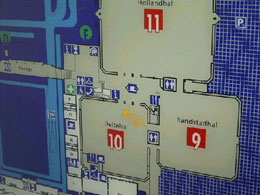
\includegraphics{images/rai_plattegrond.jpg}
\end{center}
\caption{Voorbeeld van een plattegrond (RAI)}
\label{figuur:rai_plattegrond}
\end{figure}

\item In vrijwel alle ruimtes vinden we blauwe bordjes voor faciliteiten als garderobe, WC, brandblussers en naar andere hallen en zalen. Deze bordjes zijn voorzien van pijltjes om de richting aan te geven.
\item In enkele gangen hangen electronisch programmeerbare borden. Deze bieden slechts een minieme ondersteuning en zijn erg beperkt programmeerbaar.
\end{itemize}

\item \emph{Evenement-specifieke bewegwijzering}

\begin{itemize}
\item Buiten staan grote blauwe zuilen waarin voor ieder evenement borden geschoven kunnen worden (zie figuur~\ref{figuur:rai_zuil}).

\begin{figure}
\begin{center}
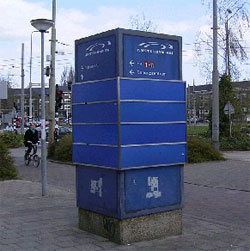
\includegraphics{images/rai_zuil.jpg}
\end{center}
\caption{Voorbeeld van een zuil (RAI)}
\label{figuur:rai_zuil}
\end{figure}

\item Bewegwijzering naar parkeerplaatsen verschilt ook per evenement, vooral afhankelijk van de drukte.
\end{itemize}

Overige evenement-specifieke bewegwijzering wordt niet door de RAI geregeld, maar door de organisatie van het betreffende evenement.

\item \emph{Niet-standaard bewegwijzering}

In het geval van onvoorziene omstandigheden, zoals een defecte lift, worden er door de RAI kleine witte zuilen geplaatst waarop simpele boodschppen op A4 formaat gehangen kunnen worden.

\end{itemize}


\section{AHOY Rotterdam} \label{sectie:overzicht_ahoy}

In het AHOY complex hebben de verschillende zalen en hallen ook nummers en namen. AHOY gebruikt voor de bewegwijzering echter bij voorkeur geen van deze twee. Op de borden in AHOY staan alleen de namen van de evenementen vermeld. De filosofie hier achter is dat de bezoeker niets heeft aan een zaalnummer of -naam, maar wil weten waar hij zijn of haar evenement kan vinden.

In AHOY was weinig echt permanente bewegwijzering aanwezig, behalve bordjes bij faciliteiten zoals WC, lift, garderobe, etcetera. Permanente bordjes om een richting of route te wijzen waren er vrijwel niet.

\begin{itemize}

\item \emph{Permanente bewegwijzering}

\begin{itemize}
\item Bij de ingangen van hallen en zalen hangen borden met nummer en/of naam.
\item Bij faciliteiten als WC, lift en garderobe hangen bordjes met iconen.
\item In de ruimte tussen de hallen hangen bewegwijzeringsbordjes met iconen (zie figuur~\ref{figuur:ahoy_borden}).

\begin{figure}
\begin{center}
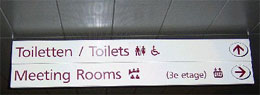
\includegraphics{images/ahoy_borden.jpg}
\end{center}
\caption{Voorbeeld van bewegwijzering (AHOY)}
\label{figuur:ahoy_borden}
\end{figure}

\end{itemize}

\item \emph{Evement-specifieke bewegwijzering}

\begin{itemize}
\item In de gangen van het complex staan verplaatsbare zuilen waarin bewegwijzerings-bordjes gehangen kunnen worden (zie figuur~\ref{figuur:ahoy_zuil}). Deze bordjes worden voor ieder evenement door de huisdrukker van AHOY gemaakt.

\begin{figure}
\begin{center}
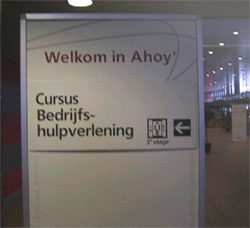
\includegraphics{images/ahoy_zuil.jpg}
\end{center}
\caption{Voorbeeld van een zuil (AHOY)}
\label{figuur:ahoy_zuil}
\end{figure}

\item In de tweede helft van 2003 hoopt AHOY electronische borden te introduceren. De bedoeling is dat deze op vaste plaatsen komen te hangen en de verplaatsbare zuilen zullen vervangen.
\end{itemize}

\end{itemize}


\section{VU Academische Ziekenhuis Amsterdam}

Hoewel in het VU Academisch Ziekenhuis eigenlijk geen echt multifunctionele ruimten zijn in dezelfde zin als dat het geval is in een beurscomplex, is de complexiteit van de bewegwijzering zeker te vergelijken. Deze bestond tijdens ons bezoek aan het ziekenhuis uit een permanent systeem van borden (dit was vrij recent ge\"\i nstalleerd) en een ge\"\i mproviseerd systeem van gele A4-tjes. Op deze gele A4-tjes werden ook tijdelijke omleidingen aangegeven.

Verschillende gebouwen worden in het ziekenhuis met letters (A t/m E), verdiepingen met nummers en kamers met nummers aangegeven.

We maken voor het VU Academisch Ziekenhuis het onderscheid tussen permanente en tijdelijke bewegwijzering, evenement-specifieke bewegwijzering is in het ziekenhuis uiteraard niet van toepassing.

\begin{itemize}

\item \emph{Permanente bewegwijzering}

\begin{itemize}
\item In veel gangen en lift-hallen hangen zilverkleurige borden met daarop gebouwletter, verdieping en reeks kamernummers (zie figuur~\ref{figuur:vu_nieuw}).

\begin{figure}
\begin{center}
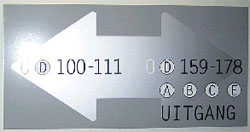
\includegraphics{images/vu_nieuw.jpg}
\end{center}
\caption{Voorbeeld van bewegwijzering (VU Ziekenhuis)}
\label{figuur:vu_nieuw}
\end{figure}

\item Door heel het complex hangen bordjes bij faciliteiten als WC en garderobe.
\item Bij ingangen van kamers zijn bordjes geplaatst met het kamernummer, omschrijving en eventueel namen van personen die in de kamer werken.
\item In sommige gangen zijn nog bordjes te vinden van het oude bewegwijzeringssysteem, waarop de gebouwen met Noord, Oost, Zuid en West aangeduid worden, in plaats van met letters (zie figuur~\ref{figuur:vu_oud}).

\begin{figure}
\begin{center}
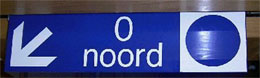
\includegraphics{images/vu_oud.jpg}
\end{center}
\caption{Voorbeeld van oude bewegwijzering (VU Ziekenhuis)}
\label{figuur:vu_oud}
\end{figure}

\end{itemize}

\item \emph{Tijdelijke bewegwijzering}

\begin{itemize}
\item Op gele blaadjes zijn gebouwletter, verdieping en reeks kamernummers met richting aangegeven.
\item Op de begane grond zijn gele blaadjes aanwezig met daarop uitgelegd hoe de inhoud van de gele blaadjes te interpreteren (zie figuur~\ref{figuur:vu_uitleg}).

\begin{figure}
\begin{center}
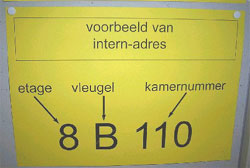
\includegraphics{images/vu_uitleg.jpg}
\end{center}
\caption{Uitleg van intern-adres (VU Ziekenhuis)}
\label{figuur:vu_uitleg}
\end{figure}

\item Een enkele keer worden witte A4-tjes met geschreven tekst gebruikt om een richting aan te geven.
\end{itemize}

\end{itemize}


\chapter{Evaluatie bestaande representaties}

We beoordelen de bestaande representaties van de drie onderzochtte complexen en proberen hier vervolgens een algemene conclusie aan te verbinden. De beoordelingen zijn gebaseerd op een congnitive walkthrough en onderzoek naar de cognitive dimensions.


\section{Cognitive walkthrough}


\subsection{De methode} \label{sectie:cw_methode}

Om de methode van cognitive walkthrough toe te passen kiezen we een stakeholder en een taak van deze stakeholder. Dit zal een taak zijn die door veel stakeholders uitgevoerd kan worden. Bij deze taak sommen we mogelijke acties op die samen tot het volbrengen van de taak kunnen leiden.

Deze acties projecteren we vervolgens op de representatie. We kijken per actie of de gebruiker merkt dat deze mogelijk is, of de gebruiker bedenkt dat deze actie ook echt een juiste is, en of de gebruiker merkt dat het goed gaat nadat hij de actie uitgevoerd heeft.


\subsection{Toepassing} \label{sectie:cw_toepassing}

De cognitive walkthrough passen we toe op de bezoeker van een evenement (zie \ref{sectie:stkh_bzkr} voor deze stakeholder) met de taak het vinden van een toilet. Omdat deze taak erg algemeen is, is hij voor veel stakeholders relevant en dus erg geschikt voor de cognitive walkthrough. Voor de verschillende bestaande representaties gebruiken we deze zelfde stakeholder en taak om de cognitive walkthrough toe te passen.


\subsection{RAI Amsterdam}

We bespreken de volgende acties die nodig zijn om het doel te bereiken in de RAI met de huidige bewegwijzering:


\subsubsection{Huidige locatie bepalen}

In de RAI hangen in iedere ruimte en bij alle in- en uitgangen plattegronden van het complex. Op een plattegrond wordt met een geel handje aangegeven waar je je op dat moment bevindt. Dit werkt met de bewegwijzering die de RAI hanteert vrij goed. Daarbij zijn de borden situatie-gericht, zodat je je ook meteen kunt ori\"enteren in welke richting je kijkt en je dus beter kunt bepalen waar je heen moet lopen.

Wat niet wordt aangegeven is op welke verdieping je je bevindt. Dit zorgt voor verwarring in bepaalde situaties, wat in het ergste geval zelfs kan betekenen dat je niet kunt vinden wat je zoekt.

In de hallen hangen in het midden aan het plafond grote vanen met daarop het halnummer. Binnen een hal kun je dus altijd gemakkelijk zien om welke hal het gaat.


\subsubsection{Locatie van doel bepalen}

Op de plattegrond wordt met iconen gewerkt. Voor toiletten worden een mannetje en vrouwtje die naast elkaar staan gebruikt. Indien er ook een invalide-toilet aanwezig is, wordt dat aangegeven met een mannetje in een rolstoel. Deze iconen staan duidelijk aangegeven op de plattegrond, dus het is makkelijk om te bepalen waar een toilet is.


\subsubsection{Route naar doel bepalen}

Omdat je gemakkelijk je huidige locatie en de locatie van je doel kunt bepalen, is het niet moeilijk een route uit te stippelen. Sowieso is het in de RAI niet echt moeilijk een toilet te vinden, omdat er vrij veel zijn. Hierdoor hoef je altijd maar weinig hindernissen te nemen (zoals in- en/of uitgangen vinden).

Maar hier komt wel weer het probleem naar voren van het slecht aangeven op welke verdieping je je bevindt (en je doel). Je kunt dus vrij lastig inschatten of je route langs een trap of lift moet lopen.


\subsubsection{Bepalen of het doel bereikt is}

Op de deuren van de WC's hangen bordjes met een mannetje, vrouwtje, of rolstoel erop, die aangeven voor welke groep mensen het toilet bedoeld is. Aan de hand van die bordjes kun je ook snel zien dat je je doel bereikt hebt. Ook bij de alle ingangen van de hallen zijn bordjes met het halnummer aanwezig.


\subsection{AHOY Rotterdam}

We bespreken de volgende acties die nodig zijn om het doel te bereiken in AHOY met de huidige bewegwijzering:


\subsubsection{Huidige locatie bepalen}

In de hallen van AHOY zijn op de wanden halnummers aangebracht, binnen een hal is het dus niet moeilijk uit te zoeken waar je bent. De hallen liggen rond een centraal gebouw, dat, afgezien van grote evenementen in het Sportpaleis, de ingang biedt voor alle evenementen. Verder zijn er geen gebouwen, dus wanneer je je niet in een hal bevindt is het ook niet moeilijk meer.

In AHOY zijn geen plattegronden te vinden, ook niet bij de ingangen. Dit is echter geen groot gemis, door de veel eenvoudiger opbouw van het complex dan bij de RAI Amsterdam het geval is.


\subsubsection{Locatie van doel bepalen}

Door het ontbreken van plattegronden kun je niet direct zien waar je doel zich bevindt, tenzij het binnen je gezichtsveld ligt. Om je route te bepalen ben je dus afhankelijk van de richtingen die door de bewegwijzering worden aangegeven.


\subsubsection{Route naar doel bepalen}

Zoals hierboven naar voren kwam wordt je route bepaald door de bewegwijzering. Gelukkig geeft deze erg goed de richting aan van vrijwel alles. Wordt je doel niet aangegeven, dan loop je vanzelf naar de centrale hal waar de richting wel wordt aangegeven.

Op de borden wordt alles aangegeven met tekst en eventueel een icoon. Daarnaast wordt erbij vermeld op welke verdieping je moet zijn wanneer dit niet de begane grond is en of het bord je richting een roltrap of lift stuurt.

Wanneer je de locatie van een evenement zoekt wordt het nog gemakkelijker. Je hoeft geen halnummer of verdieping te weten, alles wordt aangegeven met de naam van het evenement. Er staan zuilen bij de ingang en roltrappen met daarop de namen van evenementen en de richting. Wederom wordt de etage erbij vermeld en staan er eventuele iconen voor roltrap of lift.


\subsubsection{Bepalen of doel bereikt is}

Bij alle faciliteiten zoals toilet, garderobe, parkeerautomaat en lift hangen bordjes met iconen en/of tekst. In het geval van de toiletten hangen er iconen van mannetjes, vrouwtjes en rolstoelen. Ook bij de ingangen van de hallen wordt het halnummer vermeld. In het geval van een evenement wordt ook de naam hiervan gebruikt.


\subsection{VU Academisch Ziekenhuis Amsterdam}

We bespreken de volgende acties die nodig zijn om het doel te bereiken in het VU Ziekenhuis met de huidige bewegwijzering:


\subsubsection{Huidige locatie bepalen}

In het VU ziekenhuis kom je als eerste bij een informatiebalie. Verder is er een algemeen becijferingssysteem voor alle kamers die eerst bestaat uit de verdieping waar je moet zijn dan de afdeling en dan het specifieke kamernummer. Het ziekenhuis is dan opgedeeld in de afdelingen A t/m D. In het hele ziekenhuis hangen allemaal borden met pijlen gericht naar de verschillende afdelingen met verder nog specifiekere borden, als je al op een afdeling bent, waar de verschillende kamers liggen (bijvoorbeeld de kamers 100-111). Er wordt hier verder niet met plattegronden gewerkt, wel is er een algemene plattegrond die alleen de afdelingen weergeeft. Specifieker is ook niet mogelijk vanwege de complexe structuur van het ziekenhuis. Verder heb je bij omleidingen nog gele blaadjes met richtingen voor als de normale route niet te gebruiken is, deze geven meteen de specifiekere locatie aan zoals eerder beschreven.


\subsubsection{Locatie van doel bepalen}

Om de locatie van het doel te bepalen ga je bij de ingang naar de informatiebalie. Hier geef je aan wat je doel is en zij vertellen dan waar je moet zijn, je krijgt dan dus de verdieping met de afdeling en het kamernummer. Verder nog kort een uitleg over welke richting je in ieder geval op moet.


\subsubsection{Route naar doel bepalen}

De route wordt deels bepaald door de begin richting en de korte uitleg die je bij de informatiebalie hebt gekregen. Verder zie je de borden naar welke afdeling je moet. Je gaat dan eerst naar de juiste afdeling waar je dan moet zijn (op iedere afdeling zijn liften om naar een andere verdieping te gaan). Vervolgens naar de juiste verdieping, daar volg je dan de specifiekere borden naar de juiste kamers waar je vervolgens het juiste nummer zoekt.


\subsubsection{Bepalen of doel bereikt is}

De vordering in je zoek actie merk je door dat je steeds specifiekere aanduidingen krijgt van je doel. Het is ook lastig om van te voren een route uit te stippelen als je het gebouw niet echt kent. Het enige dat van te voren te plannen is, is de informatie die je vraagt bij de informatiebalie bij de entree.


\section{Cognitive dimensions}

Verschillende cognitieve dimensies projecteren we op de bewegwijzering van de RAI Amsterdam, AHOY Rotterdam en het VU Academisch Ziekenhuis Amsterdam. We noemen de positieve en negatieve punten van de systemen.


\subsection{Belangrijkste dimensies} \label{sectie:cd_demensies}

We zullen de belangrijkste cognitieve dimensies hier opnoemen en kort uitleggen wat ermee bedoeld wordt:


\begin{itemize}

\item \emph{Viscosity}

De moeite die gedaan moet worden om (kleine) wijzigingen in het systeem aan te brengen.

\item \emph{Hidden dependencies}

Afhankelijkheden tussen delen van de representatie die niet direct zichtbaar zijn.

\item \emph{Premature commitment}

Het dwingen van de gebruiker tot een beslissing voor de juiste hoeveelheid informatie voor hem/haar beschikbaar is doordat de volgorde van acties vast ligt.

\item \emph{Abstractions}

Het groeperen van entiteiten om de viscositeit te verlagen of om de representatie beter aan te laten sluiten bij de gebruiker.

\item \emph{Secondary notation}

Informatie die aan de representatie toegevoegd wordt terwijl deze geen wezenlijk deel uitmaakt van het gerepresenteerde maar het bijvoorbeeld gemakkelijker maakt de representatie te interpreteren.

\item \emph{Visibility \& Juxtaposibility}

Visibility is het gemak waarmee onderdelen van de representatie te zien zijn. Juxtaposibility is het gemak waarmee deze onderdelen te vergelijken zijn.

\end{itemize}


\subsection{RAI Amsterdam} \label{sectie:cd_rai}

We bespreken de bewegwijzering van de RAI middels de cognitive dimensions:


\subsubsection{Viscosity}

De RAI heeft op erg veel plekken plattegronden hangen. Dit is erg gemakkelijk voor de bezoeker om z'n weg te vinden, maar voor de beheerder lastig in onderhoud. Want stel dat de ``Europahal'' (Hal 1) van naam zou veranderen in ``Amerikahal'', dan houdt dat ook in dat op alle plattegronden die ene naam gewijzigd moet worden. Ook simpele tijdelijke omleidingen of defecte liften kunnen natuurlijk niet altijd bijgewerkt worden op plattegronden. Dit geldt in minder mate ook voor de andere bordjes van de bewegwijzering. De RAI lost dit op door het gebruik van de verplaatsbare zuilen (zie \ref{sectie:overzicht_rai}). Electronische borden zouden hier goed van pas kunnen komen.


\subsubsection{Hidden dependencies}

De notatie van toiletten op de plattegrond is afhankelijk van de bordjes die op de deuren hangen die aangeven dat er daadwerkelijk toiletten zijn achter die deuren. Als je deze bordjes weghaalt van de deuren, dan stellen de notaties op de plattegronden ook weinig meer voor.


\subsubsection{Premature commitment}

Doordat er geen verschil in verdiepingen wordt aangegeven, kan een bezoeker door een premature commitment onverwacht langer over de route naar zijn/haar doel doen. Een bezoeker kan volgens de plattegrond recht op zijn/haar doel aflopen, maar er eigenlijk een verdieping boven of onder zitten. Hierdoor is de bezoeker verplicht eerste een trap te vinden om op de goede plek terecht te komen. Als de bezoeker van te voren had geweten dat hij een verdieping omhoog of omlaag had gemoeten, had hij zijn/haar route anders kunnen plannen en mogelijk korter.


\subsubsection{Abstractions} \label{sectie:cd_rai_abstractions}

Op de plattegrond van de RAI is sprake van abstractie. Het icoon met koffiekopje staat voor meer dan alleen koffie (namelijk ook andere dranken). Door deze groep entiteiten te groeperen tot een icoon is de viscositeit verlaagd.


\subsubsection{Secondary notation}

De plattegrond bestaat in principe uit lijnen, maar door kleuren toe te voegen wordt het geheel veel duidelijker. Helaas is er geen secondaire notatie gebruikt om het verschil in verdiepingen aan te geven.


\subsubsection{Visibility \& Juxtaposibility}

De visibility is in orde, op de plattegrond is alles te vinden wat naar onze mening nodig is om kamers en hallen te vinden. Alles is onder gebracht in een kaart, zodat je nooit lang bezig bent met zoeken.

Om deze reden is ook de juxtaposibility goed. Alles is makkelijk te vergelijken omdat alles dicht bij elkaar op de kaart staat.


\subsection{AHOY Rotterdam}

We bespreken de bewegwijzering van AHOY middels de cognitive dimensions:


\subsubsection{Viscosity}

Doordat in AHOY zoveel mogelijk gewerkt wordt met namen van evenementen in plaats van met halnummers en/of -namen is de viscositeit van de bewegwijzering relatief hoog. Voor ieder evenement moeten opnieuw bordjes gedrukt worden die vervolgens in de verplaatstbare zuilen geplaatst worden. Electronische borden zouden hier een verbetering kunnen zijn\footnote{Eind 2003 introduceert AHOY electronische bewegwijzering, zie ook \ref{sectie:overzicht_ahoy}}.


\subsubsection{Hidden dependencies}

AHOY gebruikt geen plattegronden, het gevaar van hidden dependencies zoals genoemd bij de RAI Amsterdam in \ref{sectie:cd_rai} is hier dan ook niet zo zeer aanwezig.


\subsubsection{Premature commitment}

Ook het gevaar van premature commitments is niet direct aanwezig met de bewegwijzering van AHOY. Verdiepingen worden keurig aangegeven en doordat namen van evenementen gebruikt worden is de kans dat de bezoeker een richting moet kiezen voor hij weet in welke hal zijn/haar evenement zich bevindt ook tot een minimum beperkt.


\subsubsection{Abstractions}

Uiteraard worden er abstractions gebruikt in de iconen van de bewegwijzering. Dit zijn standaard abstractions en zijn dus direct duidelijk. Het gebruik van namen van evenementen in plaats van halnummers en/of -namen om de richting te wijzen kan ook gezien worden als een abstraction.


\subsubsection{Secondary notation}

Vaak wordt er op borden gebruik gemaakt van een extra icoon, bijvoorbeeld een roltrapje terwijl al een andere verdieping aangegeven wordt. Dit maakt het interpreteren makkelijker en geeft de gebruiker tevens enige feedback, in dit voorbeeld zal de gebruiker zeker van zijn/haar zaak zijn wanneer hij/zij een roltrap op loopt.


\subsubsection{Visibility \& juxtaposibility}

Borden bij ingangen van faciliteiten en hallen zijn duidelijk te zien. Bewegwijzering is ook duidelijk boven gangpaden gehangen, dus met de visibility zit het goed.

Bewegwijzeringborden hangen altijd recht naast en/of onder elkaar, zodat de hele groep in een oogopslag te bekijken is.


\subsection{VU Academisch Ziekenhuis Amsterdam}

We bespreken de bewegwijzering van AHOY middels de cognitive dimensions:


\subsubsection{Viscosity}

Het VU ziekenhuis heeft juist een nieuw bewegwijzeringssysteem met allemaal nieuwe borden die goed te zien zijn. De bezoeker kan zo makkelijk vinden waar hij moet zijn. Wel moet hij zijn informatie nog krijgen bij de informatiebalie. Doordat het systeem bestaat uit een becijfering en deze informatie wordt omgezet bij de balie hoeft de bewegwijzering niet echt te veranderen. Zodra een kamer verplaatst moet deze informatie alleen veranderd worden bij de balie.

Het is dus voor de bezoeker niet heel interactief, want je moet naar de balie om je informatie te krijgen, maar voor de beheerder is het erg makkelijk om te onderhouden.


\subsubsection{Hidden dependencies}

Hier heb je alleen hetzelfde als bij de RAI. Er zijn een aantal bordjes die wijzen naar de toiletten, dit zijn er helaas niet veel. Wel zijn er veel toiletten. Maar als je een bordje weghaalt van de toilet heeft de bewegwijzering erheen ook geen nut.


\subsubsection{Premature commitements}

Dit is de dimensie van de bewegwijzering in het VU ziekenhuis die je overal ziet. Zoals namelijk al beschreven is in de cognitive walkthrough moet je eerst al een richting op gaan voordat je de hele route weet. Je moet eerst een juiste richting op gaan die gegeven wordt bij de informatiebalie en langzamerhand kom je steeds dichter bij je doel door alle borden te volgen.


\subsubsection{Abstractions}

Bij het ziekenhuis is dat door de richting te geven op de afdeling zelf naar kamernummers. Je ziet dan borden met pijlen met daaronder bijvoorbeeld de kamers 100-111. Zo weet je dat alle kamers daar zitten van 100 t/m 111.


\subsubsection{Secondary notation}

Door de letters groter en kleiner op het bord te zetten wordt het overzichtelijker zodat je eerst kijkt naar de afdeling en dan pas naar de kamers. Ook maakt de kleur het duidelijk dat het een bewegwijzeringsbord is, aangezien ze allemaal dezelfde kleur en stijl hebben.


\subsubsection{Visibility \& juxtaposibility}

Door alle bewegwijzeringsborden op een duidelijke plaatst te hangen zijn deze makkelijker te vinden. Door ook dezelfde kleur aan te houden weet je meteen dat het een bewegwijzeringsbord is. De kleur van de omleidingen zijn nog duidelijker door hun fel gele kleur, zo weet je meteen of er ergens een omleiding is of niet. Het is dan ook aan te raden om deze eerst te lezen voordat je op de orginele bewegwijzeringsborden kijkt.


\section{Emoties, creativiteit en betekenis}

We bekijken de drie bestaande representaties nog aan de hand van enkele andere kenmerken.


\subsection{RAI Amsterdam}

De bordjes van de RAI zijn in principe in het blauw uitgevoerd, en komen daarom consistent over. En om die reden zijn ze ook redelijk zakelijk; geen drukke tierelantijnen. De bordjes komen wel een beetje oubollig over. Tegenwoordig zou je eerder strakke bordjes verwachten. Ook de electronische bordjes zijn tegenwoordig veel slanker en kunnen meer tekens tegelijk weergeven.

De betekenis van de bordjes is over het algemeen duidelijk. Er was alleen een icoon die minder duidelijk overkwam en waar ook even over nagedacht moest worden wat de betekenis zou kunnen zijn. Het gaat hier over een icoon die kennelijk een mannetje met een petje moet voorstellen (zie figuur~\ref{figuur:rai_controle}). Toen dat eenmaal bedacht was, was de betekenis nog niet direct duidelijk; we twijfelen tussen kaartcontrole/portier/bewaking. Dit icoon is vooral onduidelijk omdat niet goed naar voren komt dat het hier om een persoon (of personen) gaat. Want als je dit icoon vergelijkt met het icoon voor toiletten, dan zie je daar wel meteen dat het om personen gaat. Je zou daarom ook verwachten dat dezelfde stijl zou worden aangehouden.

\begin{figure}
\begin{center}
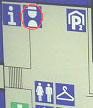
\includegraphics{images/rai_controle.jpg}
\end{center}
\caption{Icoon voor bewaking? (RAI)}
\label{figuur:rai_controle}
\end{figure}


\subsection{AHOY Rotterdam}


\subsubsection{Emoties}

Vrijwel alle onderdelen van de bewegwijzering in AHOY gebruiken een rode tekst en iconen op een witte achtergrond. Dit sluit goed aan bij de uitstraling van het complex. Alles ziet er mooi en zakelijk uit en de leesbaarheid is goed.


\subsubsection{Creativiteit}

Naast de rode tekst is er weinig opvallends te zien op creatief gebied.


\subsubsection{Betekenis}

Er wordt op veel borden naast Nederlandse tekst ook Engelse tekst gebruikt, zodat ook buitenlanders de borden begrijpen. De gebruikte iconen zijn duidelijk en vrij standaard, dus hiervan is de betekenis ook altijd duidelijk.

Richtingen worden aangegeven met pijltjes en als de roltrap of lift gebruikt moet worden wordt dat vermeld. Ook hier geen dubieuze betekenissen.


\subsection{VU Academisch Ziekenhuis Amsterdam}


\subsubsection{Emoties}

Het bewegwijzeringssysteem komt erg goed over, je hebt wel een goed gevoel over de vordering van je actie, want je komt steeds specifiekere richtingaanwijzers tegen. Het komt verder professioneel en zakelijk over. Alleen zijn er ook nog plekken waar er nog afgeweken wordt van het systeem, dat maakt het wat onoverzichtelijker en wat chaotisch. Dit ligt waarschijnlijk aan de nieuwheid van het systeem.


\subsubsection{Creativiteit}

Het systeem zelf is erg zakelijk en niet heel creatief. Wel is het systeem erg duidelijk.


\subsubsection{Betekenis}

De betekenis van de borden is erg duidelijk, wel heb je eerst een korte uitleg nodig bij de informatiebalie.  Verder weet je meteen wel wat er bedoelt wordt met de borden. Het systeem is ook overzichtelijk alleen kan je niet meteen de hele route zien.


\section{Conclusie}

De RAI gebruikt als bewegwijzering borden, iconen en plattegronden. Deze plattegronden zijn situatie gericht, wat naar onze mening een positief punt is. Aanvankelijk hadden we het idee dat dat niet zo zou zijn, maar toen we er gebruik van maakten vonden we het toch wel prettig werken.

Ook vinden we het handig dat in het midden van de hallen vanen hangen met daarop het halnummer zodat je overal in de hal duidelijk kan zien in welke hal je je bevindt.

De plattegronden vinden we niet goed wat betreft de details. Over het algemeen zijn er te veel details, het lijkt af en toe wel een bouwtekening. Maar we missen wel weer een detail: verschil in verdiepingen. De gebruikte iconen op de plattegrond zijn in orde, met als uitzondering het icoon voor kaartcontrole. Het is namelijk niet duidelijk dat het hier om een persoon gaat.

We vinden de RAI niet consistent wat betreft de aanduiding van evenementen. We zien veel tijdelijk objecten en borden. Naar onze mening zou de RAI dit zelf moeten regelen, net zoals dat ook gebeurt in de AHOY. Wat de evenementen binnen de halen ophangen en neerzetten mogen ze zelf weten, maar de bewegwijzering binnen het complex naar de evenementen toe moet de RAI zelf regelen. Dit kan waarschijnlijk het beste met digitale borden.

Verder vinden we het opvallend dat de RAI geen verwijzingen binnen het complex heeft naar toiletten, maar hebben ze alleen iconen op de plattegrond. In het VU ziekenhuis gebeurde dit ook niet (en dat vonden we een groot gemis), maar in de AHOY juist wel. Toch vinden we het niet positief of negatief, er valt namelijk voor beide systemen wat te zeggen. In de RAI zijn veel toiletten en voordat je bij je hal bent aangekomen ben je er waarschijnlijk al 1 of 2 tegengekomen.


\paragraph{Positieve punten}

\begin{itemize}
\item situatie gerichtheid van de plattegronden
\item vanen in de zalen geven goed aan in welke zaal je je bevindt
\end{itemize}


\paragraph{Negatieve punten}

\begin{itemize}
\item betekenis van 1 icoon niet duidelijk
\item plattegrond bevat te veel details
\item plattegrond maakt geen verschil in verdiepingen
\item niet consistent met aanduiding evenementen: veel tijdelijke objecten en borden
\item RAI regelt de bewegwijzering binnen het comlex naar het evenement toe niet zelf
\end{itemize}


\paragraph{Overige punten}

\begin{itemize}
\item toiletten worden alleen aangegeven op de plattegrond, er zijn geen pijlen in de gangen die ernaar wijzen
\end{itemize}


\chapter{Voorstel nieuwe bewegwijzering}

We zijn bij het bestuderen van de bestaande bewegwijzering in de RAI, AHOY en het VU Ziekenhuis een aantal interessante zaken tegen gekomen. Met als doel het aanpakken van de negatieve punten van de huidige bewegwijzering in de RAI ontwerpen we een nieuw systeem. Indien nodig kijken we hierbij naar de andere twee bestaande systemen.


\section{Eisen}

Uitgaande van de negatieve punten van het huidige systeem in de RAI komen we tot de volgende aanvullende eisen voor een nieuw systeem:

\begin{enumerate}
\item Verschil in verdiepingen moet duidelijker zijn \label{eis:verdiepingen}
\item Indien er plattegronden gebruikt worden moeten deze duidelijke iconen hebben en weinig details bevatten \label{eis:plattegronden}
\item De bewegwijzering moet consistent zijn, dit geldt voor permanente \emph{en} evenement-specifieke bewegwijzering \label{eis:consistentie}
\item Het systeem moet niet afhankelijk zijn van plattegronden \label{eis:afhankelijkheid}
\end{enumerate}

Uiteraard hebben we met meer eisen te maken, bijvoorbeeld eisen waaraan al prima voldaan wordt in de huidige bewegwijzering, of triviale eisen zoals duidelijke betekenis van iconen, juistheid van richting aanwijzers, etc.


\section{Onderdelen}

Ons voorstel voor een nieuwe bewegwijzering bestaat uit de volgende onderdelen:

\begin{itemize}
\item Borden met halnummer bij de ingang van iedere hal
\item Electronische borden bij de ingang van iedere hal waarop de naam van het evenement wordt weergegeven
\item Iconen bij de toiletten, garderobes, liften, EHBO posten, etc.
\item Borden boven de uitgangen van iedere hal met daarop nummers van de hallen waarvoor je de betreffende uitgang gebruikt
\item Iconen boven de uitgangen van iedere hal voor relevante faciliteiten
\item Borden waarop de richting aangegeven wordt naar alle hallen op een aantal strategische punten
\item Iconen met daarbij de richting aangegeven naar faciliteiten op een aantal strategische punten
\item Vereenvoudigde plattegronden op een aantal strategische punten
\item Een groot electronisch overzicht in de aankomsthal van alle evenementen met bijbehorende halnummers
\item Vanen aan het plafond van alle hallen met daarop het halnummer
\end{itemize}

We bespreken deze onderdelen en geven aan wat de voordelen en nadelen zijn ten opzichte van eventuele alternatieven. Ook wordt vermeld aan welke van de door ons gestelde eisen het onderdeel voldoet.


\subsubsection{Borden met halnummer bij de ingang van iedere hal}

Misschien wel het belangrijkste onderdeel van de bewegwijzering. Het moet bij de ingang duidelijk zijn om welke ingang het gaat, anders zal niemand er naar binnen gaan.

We hebben gekozen om halnummers te gebruiken op de permanente borden. Halnamen zijn lastiger te onthouden voor eenmalige bezoekers.

Deze borden helpen de gebruiker te bepalen waar ze zich bevinden en eventueel de locatie van hun doel te bepalen, in het geval ze er dichtbij zijn.


\subsubsection{Electronische borden bij de ingang van iedere hal waarop de naam van het evenement wordt weergegeven}

Naast het halnummer moet bij de ingang van ieder hal ook aangegeven worden welk evenement er plaats vindt. Dit is waar de bezoeker het eerst op af zal gaan.

Omdat de evenementen tijdelijk aanwezig zijn in een hal, gebruiken we hiervoor electronische programmeerbare borden. Het programmeren gebeurt in een centraal systeem, dat voor de juiste weergave op alle electronische borden van ons systeem zorgt.


\subsubsection{Iconen bij de toiletten, garderobes, liften, EHBO posten, etc.}

Hiervoor gelden dezelfde opmerkingen als voor het eerste onderdeel, op de halnummers na. We gebruiken iconen om faciliteiten aan te geven. Dezelfde iconen worden gebruikt in andere onderdelen van ons systeem.


\subsubsection{Borden boven de uitgangen van iedere hal met daarop nummers van de hallen waarvoor je de betreffende uitgang gebruikt}

Om van een hal naar een andere hal te gaan moet je altijd door een uitgang van de hal. Ons voorstel is dan ook om de halnummers die je bereikt door een bepaalde uitgang te gebruiken boven deze uitgang aan te geven, zodat ze vanuit heel de hal te zien zijn. Je kunt dan binnen de hal gemakkelijk zien waar je heen moet lopen voor een bepaalde hal, zelfs al sta je helemaal achterin of in het midden.

Deze borden komen tegemoet aan eis~\ref{eis:afhankelijkheid}, de bewegwijzering mag niet afhankelijk zijn van plattegronden. De route hoeft niet bepaald te worden op een plattegrond, maar wordt (in ieder geval het begin) al aangegeven binnen de hal.


\subsubsection{Iconen boven de uitgangen van iedere hal voor relevante faciliteiten}

Dezelfde redenering als bij het voorgaande onderdeel geldt ook voor het plaatsen van iconen boven de uitgangen van iedere hal. Wanneer je in een hal staat en naar het toilet moet, wil je direct kunnen zien welke uitgang je moet hebben in plaats van eerst naar een muur te moeten lopen om bewegwijzering te vinden.

En ook dit onderdeel helpt de bewegwijzering dus voldoen aan eis~\ref{eis:afhankelijkheid}.


\subsubsection{Borden waarop de richting aangegeven wordt naar alle hallen op een aantal strategische punten}

Het is niet handig en overzichtelijk om overal maar borden te hebben. Beter is om op een aantal strategische punten borden neer te zetten die de richting aangeven naar de hallen. Een strategisch punt zou een plek kunnen zijn waar meerdere hallen hun ingang hebben. Dit onderdeel voldoet aan eis~\ref{eis:afhankelijkheid}.


\subsubsection{Iconen met daarbij de richting aangegeven naar faciliteiten op een aantal strategische punten}

Net als dat je niet overal borden neer zet naar alle hallen, zet je ook niet overal borden neer naar faciliteiten. Ook hier is het verstandig om dit op strategische punten neer te zetten, zodat veel mensen tegelijk er gebruik van kunnen maken en dat toch de overzichtelijkheid gehandhaaft blijft. Dit onderdeel voldoet aan eis~\ref{eis:afhankelijkheid}.

Voor zowel het vorige onderdeel als dit onderdeel geld dat je dit kan vervangen met alleen plattegronden (zoals de RAI dat nu doet). Maar dat heeft als nadeel dat niet veel mensen tegelijk ernaar kunnen kijken. Daarom hebben we ook als eis gesteld dat de bewegwijzering niet afhankelijk is van plattegronden.


\subsubsection{Vereenvoudigde plattegronden op een aantal strategische punten}

Het is voor de bezoeker handig dat er een overzicht is van het hele complex, zodat je gemakkelijker een route kan uitstippelen en beter weet wat er komen gaat. Het is niet zo dat het de primaire bewegwijzering is, maar meer ter ondersteuning. Verder moeten er niet teveel details in zitten. Als de contouren van de hallen worden aangegeven en het verschil in verdiepingen, dan is dat meer dan genoeg. Met een pijl in een afwijkende en duidelijke kleur wordt aangegeven waar je je bevindt op de plattegrond. Dit onderdeel voldoet aan eisen \ref{eis:verdiepingen}, \ref{eis:plattegronden} en \ref{eis:afhankelijkheid}.


\subsubsection{Een groot electronisch overzicht in de aankomsthal van alle evenementen met bijbehorende halnummers}

Door een groot electronische bord in de aankomsthallen kan goed worden weergegeven welke evenementen gehouden worden, en waar ze te vinden zijn. Hierdoor ben je niet afhankelijk van bewegwijzering die georganiseerd wordt door het evenement, en creeer je een consistente omgeving. Daarnaast hebben electronische borden het voordeel dat ze makkelijk gewijzigd kunnen worden en dus makkelijk in onderhoud zijn. Dit onderdeel voldoet aan eis~\ref{eis:consistentie}.


\subsubsection{Vanen aan het plafond van alle hallen met daarop het halnummer}

Het is handig om in de hallen aan het plafond vanen te hangen met het halnummer erop. Zo kan iedereen die op dat moment in de hal aanwezig is zien waar diegene zich bevindt. Je zou het ook op een van de muren kunnen zetten, maar waarschijnlijk is de visibility dan lager. Je moet dan gaan zoeken naar de muur waar het nummer op staat. Dit onderdeel voldoet aan eis~\ref{eis:afhankelijkheid}.


\section{Iconen}

\begin{figure}
\begin{center}
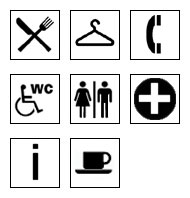
\includegraphics{images/iconen.jpg}
\end{center}
\caption{Overzicht van iconen}
\label{figuur:iconen}
\end{figure}

We gebruiken voor de faciliteiten iconen, zie figuur~\ref{figuur:iconen}. Dit omdat iconen internationaal beter werken dan woorden en minder ruimte innemen. Voor de faciliteiten waar we iconen voor gebruiken bestaan al veel min of meer ``standaard'' representaties. Het is belangrijk dat we deze gebruiken in plaats van andere creatieve oplossingen te bedenken. De bezoekers herkennen de standaard iconen direct en de betekenis is duidelijk.

De gebruikte iconen conflicteren niet met elkaar en zijn ook van een grote afstand goed herkenbaar. Daarnaast passen ze allen in dezelfde stijl.


\section{Electronisch systeem}

Het grote voordeel van electronische borden is dat je gemakkelijk met informatie om kan gaan. Je voert een keer in dat in hal 9 de AutoRAI gehouden wordt, en op alle borden waar dat op weergegeven moet worden kunnen het dan weergeven. Het is dan wel noodzakelijk dat de borden centraal beheerd worden door slimme software.
Een ander voordeel is dat je typefouten kunt verbeteren, of nieuwe namen van evenementen gemakkelijk in kunt voeren. Je hoeft niet een compleet nieuw bordje te maken (maal het aantal plaatsen waar het bordje geplaatst moet worden).

Wanneer dit mogelijk is moet het uiterlijk van de electronische borden zoveel mogelijk aansluiten bij de andere bewegwijzering.


\chapter{Evaluatie voorstel bewegwijzering}

We evalueren de door ons voorgestelde nieuwe bewegwijzering voor de RAI. Dit gebeurt net als bij de evaluaties van de bestaande systemen middels een cognitive walkthrough en een analyse op basis van cognitive dimensions. Tevens presenteren we voor deze nieuwe bewegwijzering een scenario.


\section{Cognitive walkthrough}

We gebruiken de methode van cognitive walkthrough, zoals deze uitgelegd is in \ref{sectie:cw_methode}. Wederom passen we de methode toe op de stakeholder en taak zoals uiteengezet in \ref{sectie:cw_toepassing}.

We bespreken de volgende acties die nodig zijn om het doel te bereiken in de RAI met de door ons voorgestelde nieuwe bewegwijzering:


\subsubsection{Huidige locatie bepalen}

Het bepalen van de huidige locatie is erg gemakkelijk binnen de hallen, omdat daar de vanen met halnummers hangen. Er is daaruit echter niet af te leiden waar je je ten opzichte van de rest van het complex bevindt.

Bevind je je niet in een hal, dan zul je je toevlucht moeten zoeken tot een plattegrond zoals die op enkele strategische punten hangt. Je kunt aan de pijl op de plattegrond zien waar je je bevindt.


\subsubsection{Locatie van doel bepalen}

Is het doel dichtbij, dan is het direct herkenbaar aan een icoon, halnummer, of naam van evenement. Moet je verder weg zijn, dan is uit de bewegwijzering alleen op te maken welke richting je moet lopen, maar niet waar je doel zich precies bevindt. Behalve wanneer je een plattegrond raadpleegt uiteraard, daar kun je direct de locatie van je doel op bepalen.


\subsubsection{Route naar doel bepalen}

In het door ons voorgestelde systeem is het eigenlijk niet mogelijk direct de volledige route naar het doel te bepalen, maar het eerste deel van de route is altijd duidelijk.

Wanneer het doel dichtbij is, kun je het direct herkennen en is het bepalen van de route triviaal. Wanneer het doel verder weg is, krijg je steeds genoeg informatie om door te kunnen lopen. Wanneer de route verder niet duidelijk is, kom je weer een onderdeel van de bewegwijzering tegen. Je hoeft zelf dus absoluut niet na te denken en je loopt automatisch altijd de kortste route.

Uitzondering is weer het gebruiken van een plattegrond. In dat geval kun je je route uiteraard wel direct zelf bepalen.


\subsubsection{Bepalen of het doel bereikt is}

Iedere ingang van de hallen en faciliteiten is te herkennen; de hallen aan het halnummer en evenement naam, de faciliteiten aan een icoon. Hierover kan dus nooit verwarring bestaan.


\section{Cognitive dimensions}

Verschillende cognitieve dimensies projecteren we op de door ons voorgestelde nieuwe bewegwijzering van de RAI Amsterdam. We noemen de positieve en negatieve punten van de systemen. Een korte uitleg van de gebruikte demensies is te lezen in \ref{sectie:cd_demensies}.


\subsubsection{Viscosity}

Het nieuwe systeem in de RAI heeft borden op een duidelijke plek hangen de bezoeker kan snel de bewegwijzeringsborden zien. Door de digitale borden kan je ook zien welke activiteit waar is, zo heb je meteen door waar je moet zijn. De digitale borden zijn voor de beheerder ook makkelijk bij te houden en de kosten van het bijhouden bestaat alleen uit tijd en energie.

Verder zijn er kaarten aan de muren waar mensen een directe route kunnen uitstippelen naar de verschillende hallen. Er hoeft in principe verder niemand geraadpleegd te worden over de route. Als een evenement erg groot is worden er over het algemeen ook plattegronden uitgedeeld door de organisatie van het evenement bij binnenkomst, zodat de bezoekers meteen een overzicht krijgen van alle hallen.


\subsubsection{Hidden dependencies}

Hier heb je weer het geval met iconen van de toiletten. Er zijn een aantal bordjes die wijzen naar de toiletten. Maar als je zo een bordje weghaalt van de toilet heeft de bewegwijzering erheen ook geen nut. Hetzelfde is dan ook met EHBO en al die andere voorziening gerichte borden met iconen.


\subsubsection{Premature commitment}

Dit is met de wegwijzering met de pijlen naar hallen, je komt door het volgen van de borden steeds dichter bij de hal. Je hebt alleen niet zo heel erg het gevoel van vordering want de borden worden niet specifieker in aanduiding. Wel weet je dat je op het goede spoor zit, je komt namelijk de borden met de juiste aanduiding tegen als je goed zit. Als je de vooruitgang echt wil weten kan je ook op een kaart kijken die aan de muur hangt en zien hoever je van je doel bent en de hele route uitstippelen.


\subsubsection{Abstractions}

Hier heb je hetzelfde als bij de RAI (zie \ref{sectie:cd_rai_abstractions}), alleen heb je nu ook borden die naar het doel wijzen en niet alleen de plattegrond.


\subsubsection{Secondary notation}

Door alles in dezelfde kleur en stijl te doen is het duidelijk dat het gaat om een wegwijzeringsbord. De kaarten zijn verlicht en hebben een opvallende kleur zodat ze opvallen.


\subsubsection{Visibility \& juxtaposibility}

Door alle bewegwijzeringsborden op een duidelijke plaatst te hangen zijn deze makkelijker te vinden. Door ook dezelfde kleur aan te houden weet je meteen dat het een bewegwijzeringsbord is. De digitale borden geven extra informatie weer over de hal en dat valt hoe dan ook wel op door het licht.


\section{Emoties, creativiteit en betekenis}

We bekijken de door ons voorgestelde bewegwijzering nog aan de hand van deze drie kenmerken:


\subsubsection{Emoties}

Het bewegwijzeringssysteem komt goed over, je ziet iedere keer of je de goede richting op gaat ook heb je een extra hulpmiddel (de plattegronden) waarmee je een hele route kan uitstippelen. Het komt verder professioneel en zakelijk over door de digitale borden en het feit dat de alle borden dezelfde stijl hebben.


\subsubsection{Creativiteit}

Het systeem zelf is zakelijk en niet heel creatief. Wel is het systeem er duidelijk en goed doordacht en is het ontwerp wel mooi.


\subsubsection{Betekenis}

De betekenis van de borden is erg duidelijk, Door de extra informatie van de digitaleborden weet je meteen waar je moet zijn. Verder weet je meteen wel wat er bedoelt wordt met de borden. Als je zelf de borden niet meer overzichtelijk vind ondanks de duidelijkheid kan je altijd nog op de kaart kijken die je overal wel aan de muur kan vinden. Zo kan iedereen zijn weg vinden.


\section{Scenario}

Om een idee te krijgen hoe het systeem in de praktijk gebruikt zou kunnen worden schrijven we een scenario. Een willekeurige persoon voert enkele acties uit en we letten daarbij op hoe hij de door ons voorgestelde bewegwijzering gebruikt.


\paragraph{Scenario} Meneer Kievit is naar de \emph{autoRAI} en is opzoek naar de \emph{BMW} afdeling. Hij ziet bij de ingang een overzicht van alle activiteiten en vindt daar BMW, deze is in hal 9. Verder ziet hij ook gelijk de richting waar hal 9 is. Hij gaat dus naar links toe en ziet na 100 meter een bord met hal 9 erop. Bij de ingang van een hal daaronder ziet hij dan digitaal weergegeven ``BMW''. Hij gaat de hal binnen en kijkt rond.

Meneer Kievit is nu al drie uur op de beurs en bevindt zich nog steeds in hal 9 (hij weet dit door de vaan die midden in de hal hangt). Hij heeft nog niks gedronken en heeft dus erge dorst en besluit om wat te gaan drinken. Hij gaat opzoek naar een drinkgelegenheid. Hij zoekt naar een aanwijzing voor een drinkgelegenheid, hij loopt naar de uitgang van de hal en ziet daar een bordje met een kopje (koffie) erop en ziet dat als een duidelijke aanwijzing voor een plek om iets te drinken. Hij volgt het bordje en gaat dan de gang door.

Hij komt nu hal 10 binnen en ziet daar een bordje dat hij links moet gaan om bij een drinkgelegenheid te komen. Vervolgens ziet hij weer net zo'n bordje als hij bij de hoek komt van de hal en ziet dat hij naar rechts moet. Na drie bordjes ziet hij dan een drinkgelegenheid. Hij bestelt een kop koffie en wil een slok nemen, maar het kopje blijft in zijn snor haken en de koffie valt over hem heen. De koffie is nog gloeiend heet en hij heeft zich verbrand. Hij gaat snel opzoek naar een EHBO post.

Hij ziet naast zich aan de muur een kaart met een overzicht van de beurshallen, kijkt daar snel op en ziet een teken met een kruisje: een algemeen teken voor een EHBO post. Hij ziet dat hij naar een andere hal moet en gaat naar de juiste uitgang en ziet daar al een bordje met dezelfde kruis. Hij volgt dit bordje en moet dus naar de gang en dan links en ziet dan de EHBO post ook angegeven door dezelfde kruis. Hij wordt daar geholpen. Nu heeft hij genoeg van de beurs en wil weg, hij ziet al meteen een bordje met het bekende uitgangsteken en gaat zo de beurs uit naar huis.


\section{Conclusie}

Bij het ontwerpen van een bewegwijzeringssysteem moet een keuze gemaakt worden. Geef je de gebruikers het volledige overzicht en laat je ze zelf de route bepalen? Of houd je de informatie beperkt tot dat wat nodig is en kauw je de route voor voor de gebuiker? Hier ligt het belangrijkste verschil tussen de huidige bewegwijzering in de RAI en de door ons voorgestelde bewegwijzering.

Het huidige systeem geeft nauwelijks richtingen aan, maar biedt erg veel plattegronden waarmee de gebruiker zelf de richting kan bepalen. Dit gaat soms mis, bijvoorbeeld in het geval een doorgang tijdelijk niet beschikbaar is, of wanneer de verdieping niet is weergegeven op de plattegrond. Maar in de meeste gevallen werkt deze oplossing prima. Het grote nadeel is echter dat het bepalen van je eigen locatie, het bepalen van de locatie van je doel en het uitstippelen van een route daartussen tijd kost. Dit wordt extra vervelend op een drukbezochte beurs, waar de mensen zich verdringen rond de plattegronden.

Ons leek het daarom een goed idee af te stappen van de afhankelijkheid van plattegronden. Ze zijn weliswaar zeer waardevol als aanvullende bewegwijzering, voor de gebruiker die meer wil weten over het complex, maar als primaire bewegwijzering zijn ze naar onze mening minder geschikt.

Daarom hebben wij ervoor gekozen veel gebruik te maken van borden waarop richtingen aangegeven worden. De gebruiker ziet de borden, kiest de juiste, leest de richting af en loopt door. Een totaaloverzicht ontbreekt hierdoor, maar het is snel, makkelijk en effectief.

Een ander punt waarop we het de gebruiker gemakkelijker maken is de naamgeving van de hallen. We leren hier van de filosifie achter de bewegwijzering in AHOY Rotterdam: De gebruiker komt voor een evenement en heeft dus meer aan de naam van het evenement dan aan een halnummer.


\end{document}
